\documentclass[10pt]{article}
\usepackage[margin=18mm]{geometry}
\usepackage{graphicx,booktabs,array,hyperref}
\hypersetup{colorlinks=true,urlcolor=blue}
\setlength{\parindent}{0pt}\setlength{\parskip}{5pt}
\begin{document}
\section*{Native algebraic IC follow-up: measured stage results}
Report date: 2026-10-25. Status: finite stage evidence; the wider campaign is partial.

Degree-two symmetric preprocessing has fewer recorded solver words in
263 of 304 completed paired queries. Degrees three and four have more in
every completed pair. These are native count observations, not full-query
or DLP speedups. The direct hybrid's input-degree floor may reach six.

\begin{center}\begin{tabular}{rrrrl}\toprule
Closure & raw rows & complete extractions & symmetric lower & ratio range\\\midrule
2 & 1152 & 768 & 263/304 & 0.04201--5.123 \\
3 & 1152 & 891 & 0/304 & 1.342--178.5 \\
4 & 1152 & 923 & 0/304 & 13.37--1.65e+04 \\
\bottomrule\end{tabular}\end{center}

\begin{center}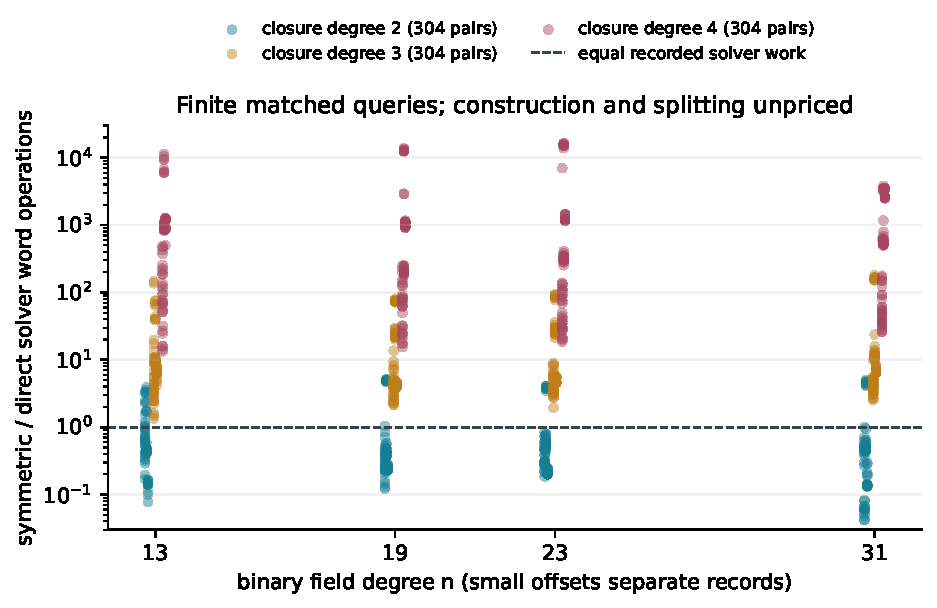
\includegraphics[width=.96\linewidth]{closure-ratios.pdf}\end{center}

All three panels use the same public targets and seeded bases at $n=13,19,23,31$,
$\ell=2,3,4$. Prefix duplicates are retained in raw data and excluded from the
primary comparison. There are 336 distinct inputs, 304 completed matched pairs;
32 incomplete pairs are excluded and remain unknown. Direct group enumeration
found no answer mismatch. The 8,100 symmetric algebraic roots in the completed
queries yielded only four verified x-multisets; 8,096 roots failed split/lift.

\newpage
\section*{Guessing, controls, and what remains}
For the balanced three-set $[7,15,23]$ at the original ell=8 draw 0,
all eight branches now saturate degree four without refuting. The rank is
129,221 on branches 0--3 and 129,473 on 4--7. This independent replay agrees
with the upstream branch-0 result and fills seven previously unmeasured
branches. It establishes failure of this set on this draw, not a global minimum.

The exact fixture oracle independently reproduces all seven original counts;
all three SAT controls have checked Boolean witnesses. Small controls cover
2,304 direct assignments, every corresponding small symmetric root, repeated
roots and 2,880 signed-lift cases. The u128 builder matches the library's actual
equations at m=3--6; sparse and parallel fixed points match the dense controls.

The first-two-summand exchange is checked on all 308 coordinate equations of
the seven original fixtures. Certificate \texttt{IDC1ha27a77e72057f9cb} also
checks S3's ordinary integer-polynomial symmetry. Its formal-proof pointer is
unset. The permutation equates degree verdicts for $[7,23,24]$ and $[15,23,24]$,
not their costs.

Original-setup failures and internal-cap refusals are retained. The first
structural outer shell ended with a syntax error after all 96 native commands
had succeeded; its amended-on-disk runner caused the tail error. Subsequent
panels execute frozen runner copies. No failed attempt is assigned zero cost.

No full-price IC gain or rho crossover is established. Complete DLP smoke,
remaining guess draws, ell=9, actual N=58/60 continuations, sparse N=100,
quartic replay/scaling, wide arithmetic and external-CAS/hardware controls
remain separate obligations. The current quartic implementation explicitly
refuses m=16--18. Source-pinned jobs and blocked backlog cards preserve them.

The owner's total additional cloud-compute ceiling is USD 100. No paid job
had been launched when this report was prepared. A read-only CI access probe
is separate from a compute allocation.

\section*{Evidence and scope}
Native recomputation: \path{examples/ic_campaign_report_data.rs}.
Raw values and audit pointers: \path{../../report-data.json}. Per-panel
reports are siblings under \path{../}. Frozen requirements and amendments:
\path{../../PROTOCOL.md}. Upstream references:
\href{https://github.com/aburan28/crypto/pull/2214}{fall-degree PR 2214};
\href{https://github.com/aburan28/crypto/pull/2429}{guessing PR 2429};
\href{https://github.com/aburan28/cryptanalysis/tree/claude/cryptanalysis-repo-setup-p59kek/experiments/pdp-degree-heuristics}{cryptanalysis structured-base study}.
Solver construction, cubic splitting, lifting, physical conversion and the
complete IC/rho pipeline are not collapsed into the plotted word ratios.

\end{document}
